\documentclass[9pt]{IEEEtran}

\usepackage[english]{babel}
\usepackage{graphicx}
\usepackage{caption}
\captionsetup{justification=justified}

\usepackage{placeins}
\usepackage{epstopdf}
\usepackage{fancyhdr}
\usepackage{amsmath}
\usepackage{amsthm}
\usepackage{amssymb}
\usepackage{url}
\usepackage{array}
\usepackage{textcomp}
\usepackage{listings}
\usepackage{hyperref}
\usepackage{xcolor}
\usepackage{colortbl}
\usepackage{float}
\usepackage{gensymb}
\usepackage{longtable}
\usepackage{supertabular}
\usepackage{multicol}
\usepackage[justification=centering]{caption}
\usepackage{amsmath}
\usepackage{subcaption}

\usepackage[utf8x]{inputenc}

\usepackage[T1]{fontenc}
\usepackage{lmodern}
\input{glyphtounicode}
\pdfgentounicode=1

\graphicspath{{./figures/}}
\DeclareGraphicsExtensions{.pdf,.png,.jpg,.eps}

% correct bad hyphenation here
\hyphenation{op-tical net-works semi-conduc-tor trig-gs}

% ============================================================================================

\title{\vspace{0ex} Bayesian Logistic Regression}

\author{Aljaž Konec\vspace{-5.0ex}}

% ============================================================================================

\begin{document}

\maketitle

\section{Introduction}
In this report we showcase the implementation of Bayesian logistic regression. 
First we compare the posterior distributions of the coefficients for all shots and subsampled shots.
Then we discuss the importance of the features and how they are linked to the probability of making a shot.

\vspace*{-0.5cm}
\section{Personal Opinion}
\vspace*{-1ex}
In our personal opinion, distance from the basket plays a more important role in the probability of making a shot than the angle of the shot.
The further away from the basket the player is, the less likely the shot is made.
Therefore we expect the coefficient $\beta_1$ to have mostly negative values.
Since players train on shooting there will be certain distances where the player is most comfortable shooting and therefore the coefficient $\beta_1$ will have a positive value.
All of this is summarized in Figure \ref{fig:personal_opinion}.
\begin{figure}[H]
    \centering
    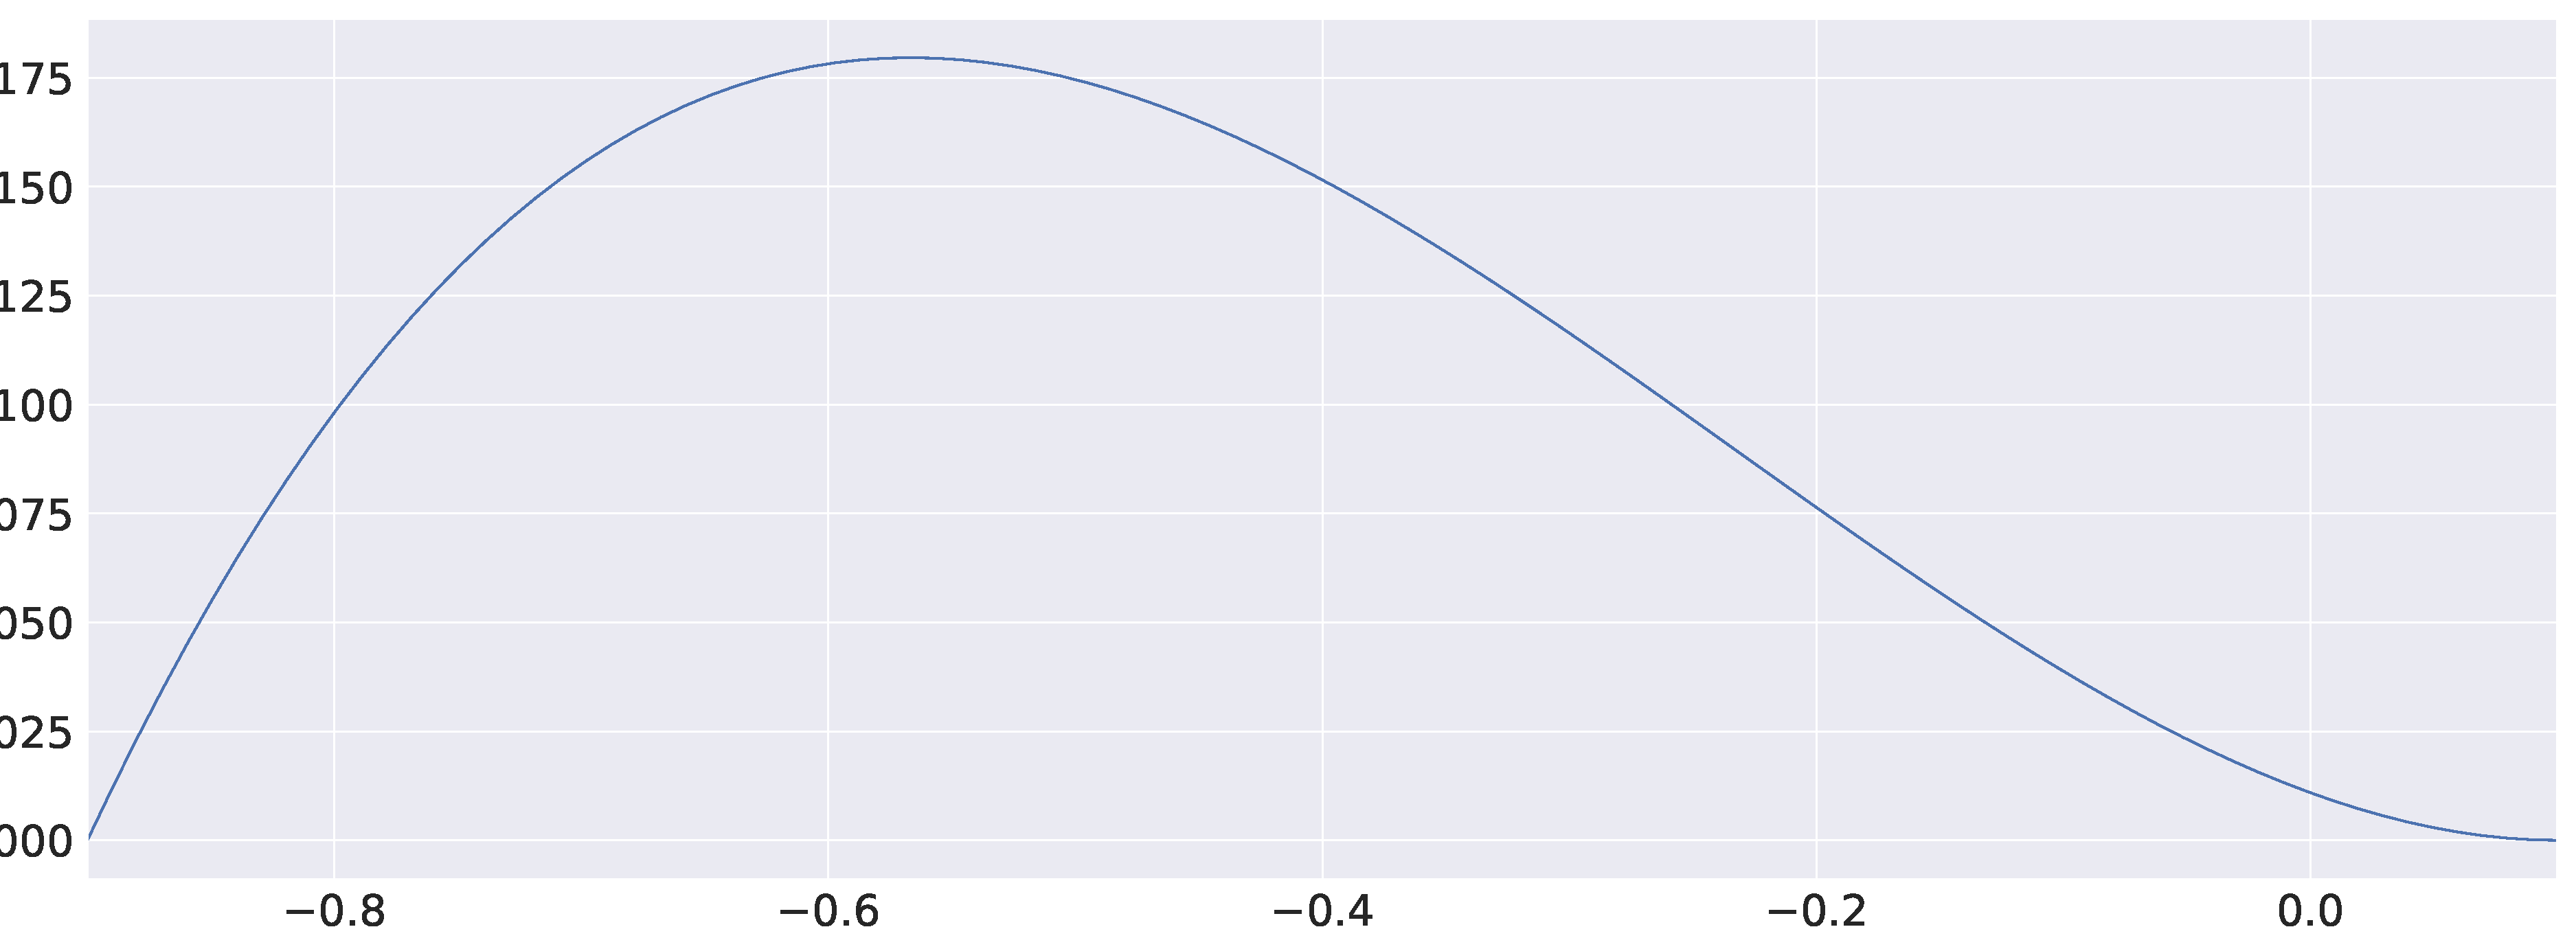
\includegraphics[width=0.5\textwidth]{personal_opinion.pdf}
    \caption{Personal opinion on the coefficient for Distance.}
    \label{fig:personal_opinion}
\end{figure}

\section{Resulting Posterior Distributions }
We perform MCMC sampling on all shots and 50 randomly subsampled shots to obtain two posterior distributions for both coefficients.
The results are shown in Figure \ref{fig:beta0}.
\begin{figure}[h]
    \centering
    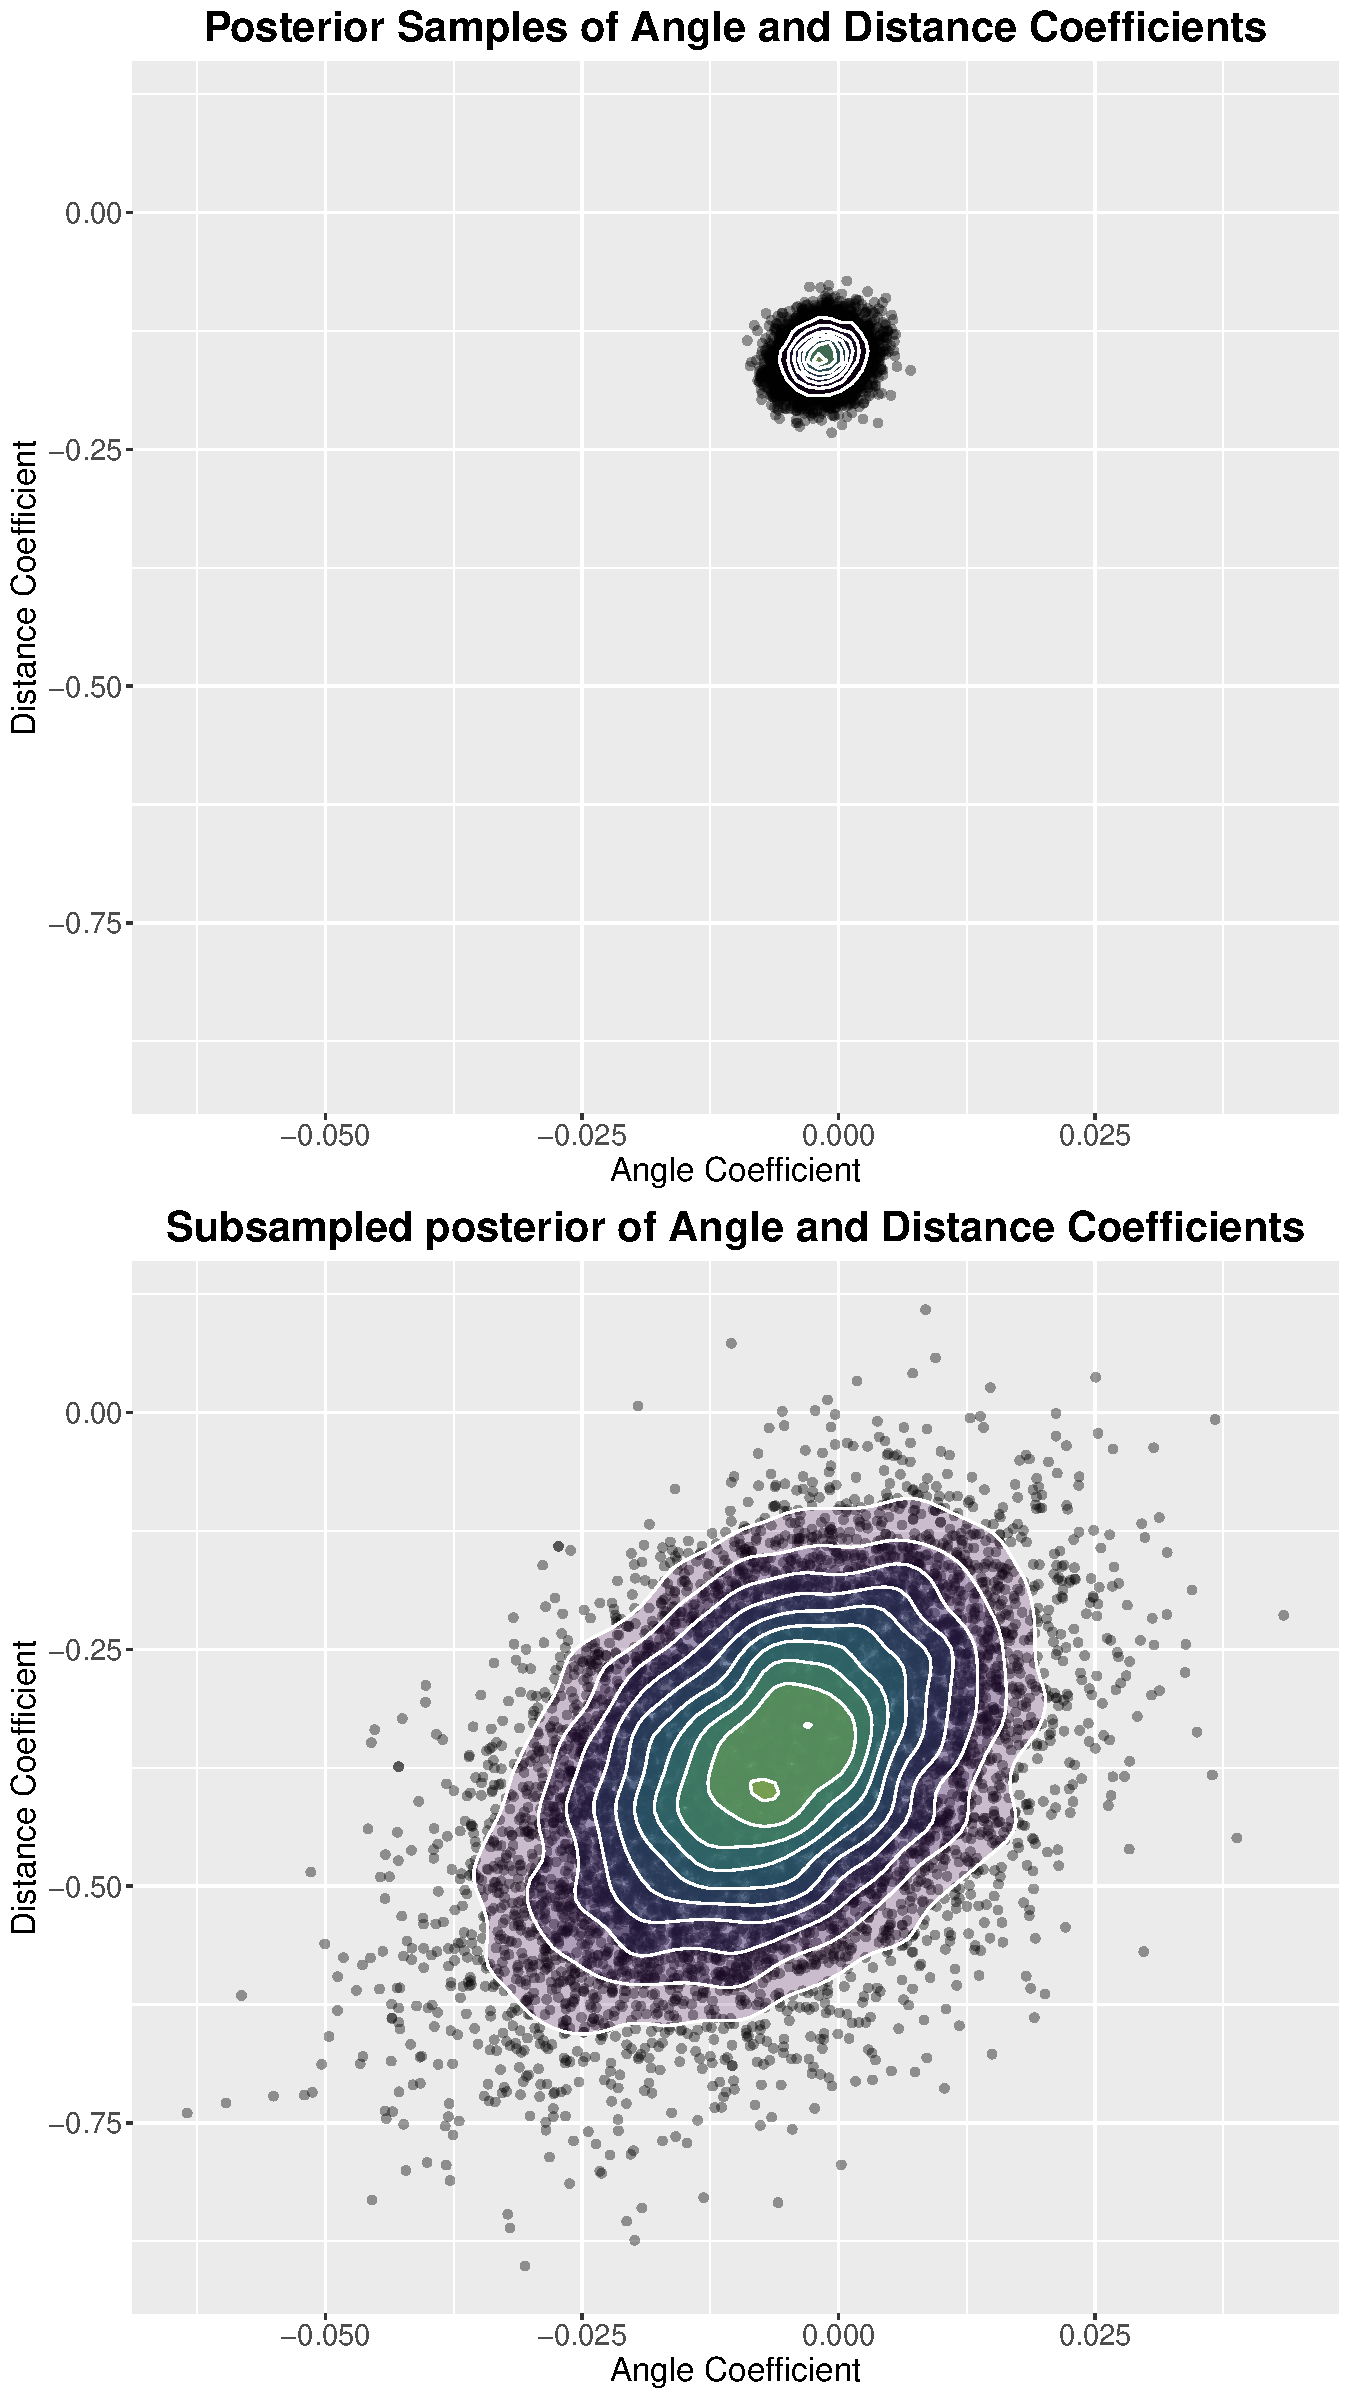
\includegraphics[width=0.4\textwidth]{combined_plot_vertical.pdf}
    \caption{Posterior distributions for angle and distance coefficients for all shots and subsampled shots.}
    \label{fig:beta0}

\end{figure}
Comparing the posterior distributions to our personal opinion we can see that the distance coefficient is infact negative just not to the extent we expected.
Infering from subsampled data results in similar distributions where the distance coefficient is negative and the angle coefficient is close to zero.

Comparing the distributions for all shots and subsampled shots it can be observed that the former gives a much smaller area of probable coefficient values.
This indicates that the the model is more certain about the coefficients when using more data.
Table \ref{tab:beta0} shows the mean and standard deviation of the posterior distributions for both coefficients.
The standard deviation for subsampled distribution is much larger, which again shows the larger uncertainty in the model when using less data.
\begin{table}[!ht]
    \centering
    \begin{tabular}{lll}
        \textbf{} & \textbf{All Data} & \textbf{Subsampled Data} \\ \hline
        \textbf{Angle Coefficient} & -0.0400 $\pm$ 0.055 & -0.1850 $\pm$ 0.3423\\ 
        \textbf{Distance Coefficient} & -0.4309 $\pm$ 0.057 & -1.0605 $\pm$ 0.3689\\ 
    \end{tabular}
    \caption{Means and standard deviations of both posterior distributions for the angle and distance coefficients.}
    \label{tab:beta0}
\end{table}

\vspace*{-0.6cm}
\section{Importance of Features}
The more important feature can be inferred from the percentage of the posterior samples where the absolute value of one coefficient is larger than the other.
This can be calculated as:
\begin{equation}
    P(|\beta_0| > |\beta_1|) = \frac{1}{N} \sum_{i=1}^{N} \mathbf{1}_{(|\beta_0| > |\beta_1|)}(\beta_0^{(i)}, \beta_1^{(i)}) = 1
\end{equation}
This indicates that the distance coefficient is more important than the angle coefficient in determining the probability of making a shot.                  


\section{Shot success based on increasing angle}
We can calculate this by calculating the probability that the angle coefficient is negative, indicating the that shot success decreases with increasing angle.
The probability can be calculated as the proportion of posterior samples that are negative:
\begin{equation}
    P(\beta_0 < 0) = \frac{1}{N} \sum_{i=1}^{N} \mathbf{1}_{(x < 0)}(\beta_0^{(i)}) = 0.7627
\end{equation}
We conclude that the coefficient of the angle is negative 76.27\% of the time, indicating that the shot success decreases with increasing angle.



\bibliographystyle{IEEEtran}
\bibliography{bibliography}

\end{document}
